%%%%%%%%%%%%%%%%%%%%%%%%%%%%%%%%%%%%%%%%%%%%%%%%%%%%%%%%%%%%%%%%%%%%%%%%%%%%%%%%%%%%%%%%%%%%%%%%%%%%%%%%%%%%%%%%%
%                                     PAPER ROMMEL - ELSY                                                       %
%%%%%%%%%%%%%%%%%%%%%%%%%%%%%%%%%%%%%%%%%%%%%%%%%%%%%%%%%%%%%%%%%%%%%%%%%%%%%%%%%%%%%%%%%%%%%%%%%%%%%%%%%%%%%%%%%

%%%%%%%%%%%%%%%%%%%%%%%% DECLARACIONES DE LIBRERIAS Y PAQUETES %%%%%%%%%%%%%%%%%%%%%%%%%%%%%%%%%%%%%%%%%%%%%%%%%
\documentclass[conference]{IEEEtran}
\IEEEoverridecommandlockouts
% The preceding line is only needed to identify funding in the first footnote. If that is unneeded, please comment it out.
\usepackage{cite} %paquete de la cita bibliografica
\usepackage{amsmath}
\usepackage{amsmath,amssymb,amsfonts} %paquete de fuente
\usepackage{algorithmic} %paquete de simbología númerica
\usepackage{graphicx} %paquete de imagenes
\usepackage{textcomp} %paquete de 
\usepackage{xcolor} %paquete de los colores en texto
\usepackage{hyperref} %paquete de link en el texto
\def\BibTeX{{\rm B\kern-.05em{\sc i\kern-.025em b}\kern-.08em
    T\kern-.1667em\lower.7ex\hbox{E}\kern-.125emX}} %paquete de estructura de las cita bibliografica
\definecolor{orcidlogocol}{HTML}{A6CE39} %paquete de un color especifico para el logo del codigo orcid.
\usepackage{flafter}
\usepackage{amsmath}
\usepackage{multirow}
\usepackage{colortbl}
\usepackage{tablefootnote}
\usepackage{booktabs}
%%%%%%%%%%%%%%%%%%%%%%%%%%%%%%%%%%%%%%%%%%%%%%%%%%%%%%%%%%%%%%%%%%%%%%%%%%%%%%%%%%%%%%%%%%%%%%%%%%%%%%%%%%%%%%%%%
%                                    INICIO DEL DOCUMENTO                                                       %
%%%%%%%%%%%%%%%%%%%%%%%%%%%%%%%%%%%%%%%%%%%%%%%%%%%%%%%%%%%%%%%%%%%%%%%%%%%%%%%%%%%%%%%%%%%%%%%%%%%%%%%%%%%%%%%%%
\begin{document}
%%%%%%%%%%%%%%%%%%%%%%%%%%%%%%%%%%%%%%%%%%%%%%%%%%%%%%%%%%%%%%%%%%%%%%%%%%%%%%%%%%%%%%%%%%%%%%%%%%%%%%%%%%%%%%%%%
%                                     TITULO Y AUTORES                                                          %
%%%%%%%%%%%%%%%%%%%%%%%%%%%%%%%%%%%%%%%%%%%%%%%%%%%%%%%%%%%%%%%%%%%%%%%%%%%%%%%%%%%%%%%%%%%%%%%%%%%%%%%%%%%%%%%%%

\title{Analyze the implementation and impact of Communication-Based Train Control (CBTC) and Automatic Train Protection (ATP) railway signaling systems on the operational improvement of railway projects in Ecuador\\
%{\footnotesize \textsuperscript{*}Note: Sub-titles are not captured in Xplore and
%should not be used}
}
\author{
    %%%%%%%%%%%%%%%%%%%%%%%% PRIMER AUTOR %%%%%%%%%%%%%%%%%%%%%%%%%%%%%%%%%%%%%%%%%%%%%%%%%
    \IEEEauthorblockN{1\textsuperscript{st} Elsy del Rocío Villamar Garcés}
    \IEEEauthorblockA{\textit{Universidad Politecnica de Madrid-ETSII}\\
    Madrid, Spain \\
    %e.villamar@alumnos.upm.es\\
    
\includegraphics[keepaspectratio,width=0.9em]{Imagenes_general/ORCIDiD_icon128x128.png}
    \href{https://orcid.org/0000-0001-7041-8611}{{orcid.org/0000-0001-7041-8611}}}
    \and
    %%%%%%%%%%%%%%%%%%%%%%%% SEGUNDO AUTOR %%%%%%%%%%%%%%%%%%%%%%%%%%%%%%%%%%%%%%%%%%%%%%%%%
    \IEEEauthorblockN{2\textsuperscript{nd} Rommel Andrés Rivera Buenaño}
    \IEEEauthorblockA{\textit{Mechanical Engineering Department}\\
    Madrid, Spain \\
    %rommelriverab@gmail.com\\
    
\includegraphics[keepaspectratio,width=0.9em]{Imagenes_general/ORCIDiD_icon128x128.png}
    \href{https://orcid.org/0009-0002-2130-5922}{{orcid.org/0009-0002-2130-5922}}}
    \and
    %%%%%%%%%%%%%%%%%%%%%%%% TERCER AUTOR %%%%%%%%%%%%%%%%%%%%%%%%%%%%%%%%%%%%%%%%%%%%%%%%%
    \IEEEauthorblockN{3\textsuperscript{rd} Javier Gómez Fernández}
    \IEEEauthorblockA{\textit{Mechanical Engineering Department}\\
    \textit{Universidad Politecnica de Madrid}\\
    Madrid, Spain \\
    %javier.gomezf@upm.es\\
    
\includegraphics[keepaspectratio,width=0.9em]{Imagenes_general/ORCIDiD_icon128x128.png}
    \href{https://orcid.org/0000-0002-3382-5776}{{orcid.org/0000-0002-3382-5776}}}
    \and
    %%%%%%%%%%%%%%%%%%%%%%%% ESPACIO HORIZONTAL PARA CENTRAR %%%%%%%%%%%%%%%%%%%%%%%%%%%%%%%%%%%%%%%%%%%%%%%%%
    %\hspace{0.25cm}
    \hspace{1.5cm}
    \hspace{1.5cm}
    \hspace{1.5cm}
    \hspace{2cm}
    %%%%%%%%%%%%%%%%%%%%%%%% CUARTO AUTOR %%%%%%%%%%%%%%%%%%%%%%%%%%%%%%%%%%%%%%%%%%%%%%%%%
    \IEEEauthorblockN{4\textsuperscript{th} Juan de Dios Sanz Bobi}
    \IEEEauthorblockA{
        \hspace{6.5cm} \textit{Mechanical Engineering Department}\\
        \hspace{6.5cm} \textit{Universidad Politecnica de Madrid}\\
        \hspace{6.5cm}Madrid, Spain \\
        %\hspace{6.5cm}juandedios.sanz@upm.es\\
        \hspace{7cm}
\includegraphics[keepaspectratio,width=0.9em]{Imagenes_general/ORCIDiD_icon128x128.png}
        \href{https://orcid.org/0000-0002-8039-8527}{{orcid.org/0000-0002-8039-8527}}
    }
}

\maketitle
%%%%%%%%%%%%%%%%%%%%%%%%%%%%%%%%%%%%%%%%%%%%%%%%%%%%%%%%%%%%%%%%%%%%%%%%%%%%%%%%%%%%%%%%%%%%%%%%%%%%%%%%%%%%%%%%%
%                                    RESUMEN                                                                    %
%%%%%%%%%%%%%%%%%%%%%%%%%%%%%%%%%%%%%%%%%%%%%%%%%%%%%%%%%%%%%%%%%%%%%%%%%%%%%%%%%%%%%%%%%%%%%%%%%%%%%%%%%%%%%%%%%
\begin{abstract}
¿Did you know that the CBTC and ATP railway signaling systems could transform the management capacity of the railway superstructure in Ecuador? ATP ensures safety through train detection, separation, and interlocking control. CBTC systems, which support several grades of automation, offer advantages in reliability, capacity, energy efficiency, and scalability compared to ATP. Using the Binary Decision Diagrams (BDD) method, this research demonstrates that CBTC outperforms ATP in terms of reliability (12.85\%), safety (10.5\%), capacity (2.8\%), maintenance (1.66\%), and costs (4.5\%). Simulations indicate that transitioning from ATP to CBTC improves capacity by optimizing headway to 30 seconds less than the theoretical value in the studied case, and enhances traffic management by adding 6 more trains to the line. This analysis concludes that adopting CBTC technology in Ecuador is a strategic investment with substantial long-term benefits in operational efficiency, safety, and reliability.
\end{abstract}

\begin{IEEEkeywords}
CBTC, ATP, ATO, ATS, Headway, Railway Signaling, UGT, GoA
\end{IEEEkeywords}

%%%%%%%%%%%%%%%%%%%%%%%%%%%%%%%%%%%%%%%%%%%%%%%%%%%%%%%%%%%%%%%%%%%%%%%%%%%%%%%%%%%%%%%%%%%%%%%%%%%%%%%%%%%%%
%                                    INTRODUCCIÓN                                                           %
%%%%%%%%%%%%%%%%%%%%%%%%%%%%%%%%%%%%%%%%%%%%%%%%%%%%%%%%%%%%%%%%%%%%%%%%%%%%%%%%%%%%%%%%%%%%%%%%%%%%%%%%%%%%%

\section{Introduction}
In the initial stages, railway signaling depended on human operators and telephonic communications to coordinate between stations, crucial for ensuring safety; however, with technological advancements, ATP systems have significantly enhanced protection, safety, and efficiency in railway operations.

\begin{figure}[htbp]
    \centering
    \centerline{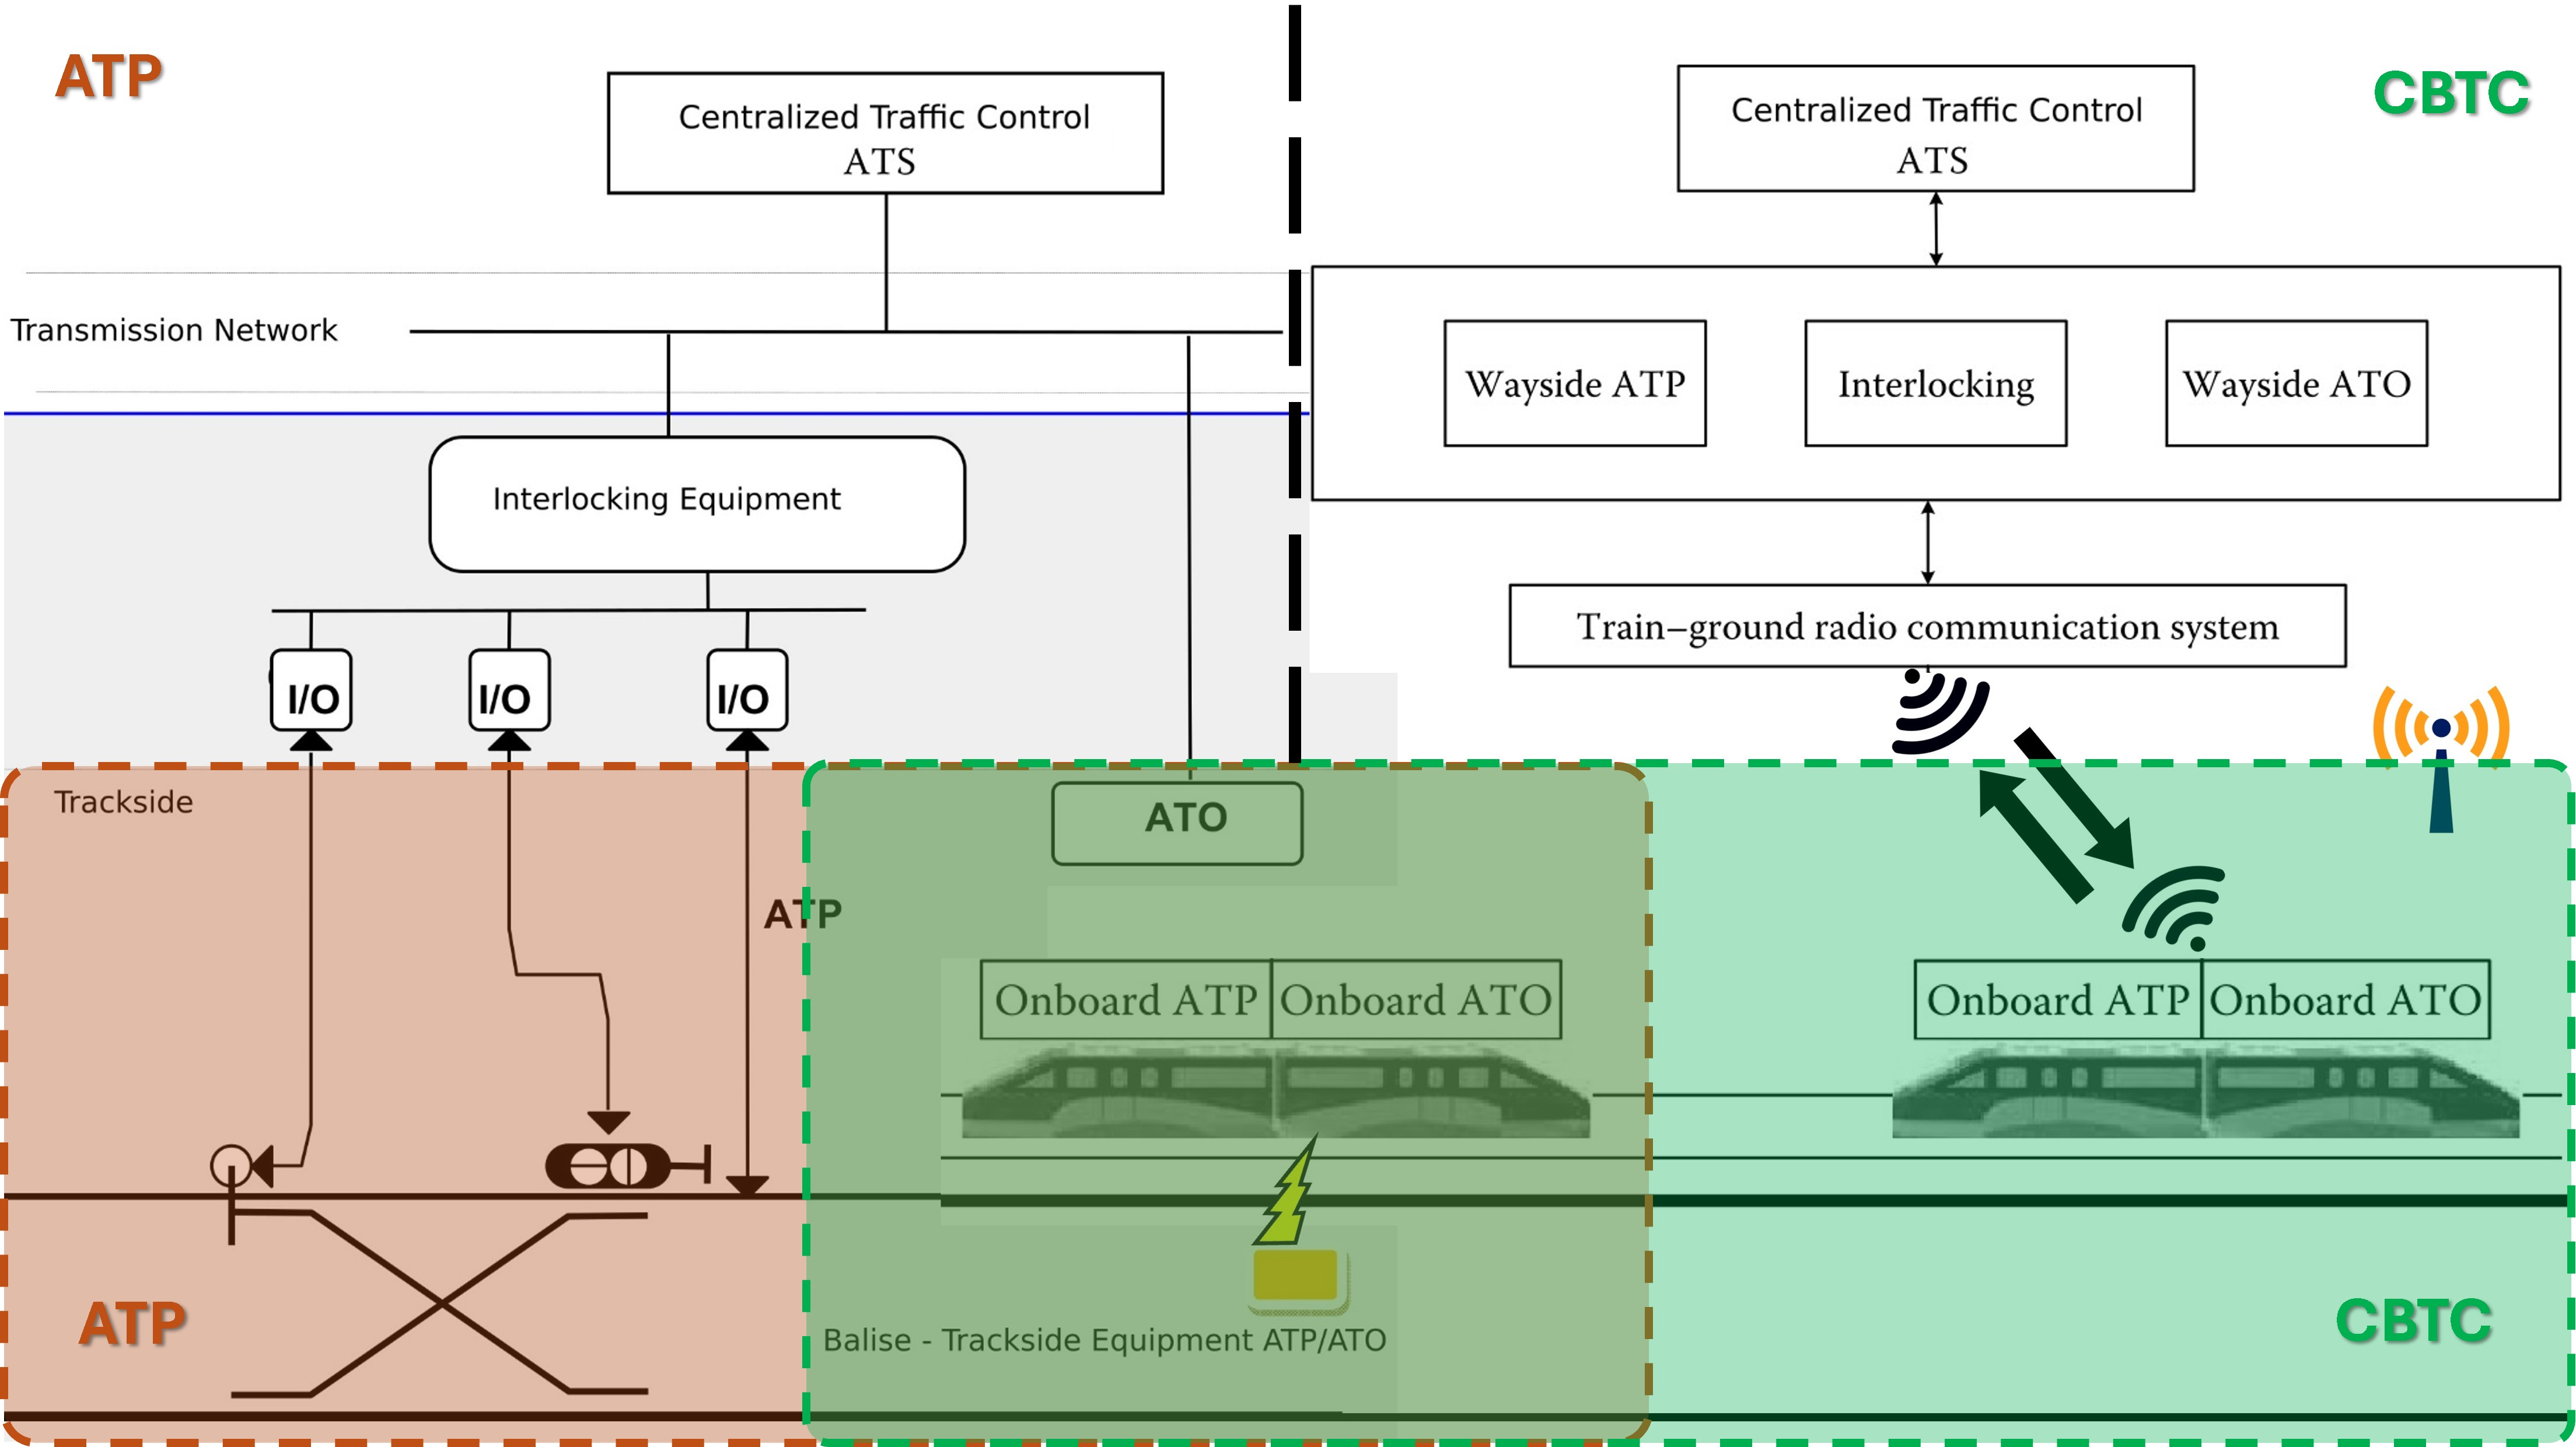
\includegraphics[width=0.45\textwidth, scale=1, angle=0]{Imagenes_general/ATP_vs_CBTC.jpg}}
    \caption{ATP and CBTC Architecture scheme}
    \label{ATP Architecture diagram}
\end{figure}

The ATP system forms the foundation of modern railway signaling systems. It has evolved to meet the critical demands for train integrity verification and precise, real-time location tracking. This is achieved through continuous communication between trackside and onboard equipment CBTC, significantly enhancing safety and efficiency on the rails. Figure [\ref{ATP Architecture diagram}]
CBTC system supports several levels of automation, including driverless train operations, and offers advantages such as increased service reliability, energy efficiency, and system scalability. This system enables more precise train control using the moving block principle, which dynamically adjusts the safe distance between trains based on their speed and braking capacity, unlike the fixed block system, which divides the track into fixed sections for safety but limits operational capacity and train proximity. As defined in the IEEE 1474.1-2004 standard \cite{b1}, the CBTC system is more detailed. Figure [\ref{ATP Architecture diagram}]

In Urban Guided Transport (UGT), the grade of automation ranges from manual to autonomous operation (GoA0 to GoA4 according to UNE-EN-62290-1 \cite{b17}), include intermediate levels of assistance and automatic operation, with variations in human intervention and the technology used.

The ATP and CBTC systems operate individually to constantly monitor the speed and location of trains, ensuring safe and adaptive operations in response to changes in traffic and track conditions, minimizing human intervention and reducing the risk of accidents. ATP ensures that trains maintain safe distances, while CBTC also allows operations at shorter intervals, increasing service frequency and optimizing the superstructure efficiency. The integration of these systems enhances diagnostics and problem resolution, facilitating faster maintenance and reducing costs.

The objectives of this article:
\begin{itemize}
\item Evaluate the current capabilities of railway signaling systems in Ecuador and determine the operational needs that could be met by implementing CBTC and ATP technologies.
\item Examine the impact of adopting CBTC and ATP systems on optimizing railway headway, aiming to significantly increase the efficiency and operational capacity of the railway systems in Ecuador.
\item Provide recommendations for identifying and categorizing the technical, financial obstacles faced by the implementation of CBTC signaling system in Ecuador Urban Guided Transport systems.
\end{itemize}

%%%%%%%%%%%%%%%%%%%%%%%%%%%%%%%%%%%%%%%%%%%%%%%%%%%%%%%%%%%%%%%%%%%%%%%%%%%%%%%%%%%%%%%%%%%%%%%%%%%%%%%%%%%%%%
%                                    SECCIONES Y DESARROLLO                                                  %
%%%%%%%%%%%%%%%%%%%%%%%%%%%%%%%%%%%%%%%%%%%%%%%%%%%%%%%%%%%%%%%%%%%%%%%%%%%%%%%%%%%%%%%%%%%%%%%%%%%%%%%%%%%%%%

\section{Railway Projects in Ecuador}

Ecuador promoted its tourist train by standing out in South America with unique scenic routes that combine diverse landscapes, cultural heritage, and authentic experiences. The primary railway projects that have been fully promoted and implemented are: \cite{b2}. 

\subsection{Regional train}
The regional railway in Ecuador, inaugurated in the 19th century which relays on axles counters that allows train detection,  connects various cities and regions of the country as shown in Figure [\ref{fig:timeline_train_reg}]
\begin{figure}[htbp]
    \centering
    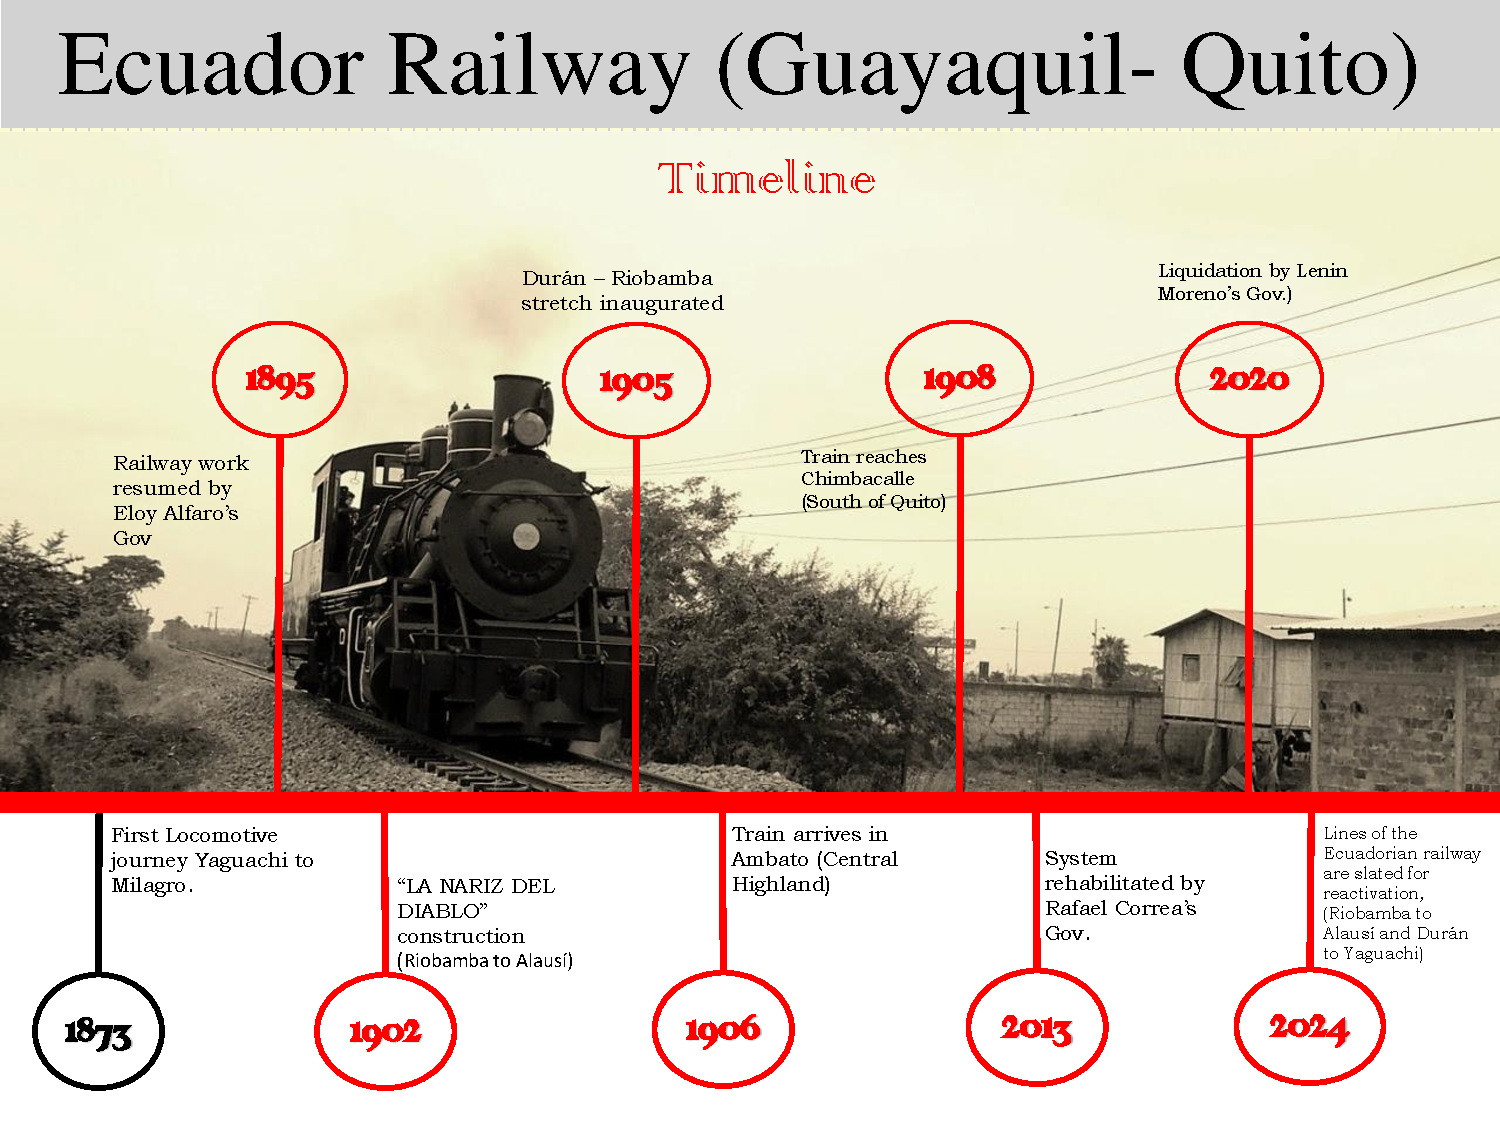
\includegraphics[width=0.45\textwidth, scale=1]{Imagenes_general/Timeline railway Guayaquil - Quito_1.pdf}
    \caption{Timeline Ecuadorian Regional train}
    \label{fig:timeline_train_reg}
\end{figure}

\subsection{Tramway de los Cuatro Rios}
The Cuenca tram \cite{b3} connects various points in the city and features third rail power supply and signaling based on electronic interlockings; its timeline is as follows: Figure [\ref{fig:timeline_train_cu}]
\begin{figure}[htbp]
    \centering
    \includegraphics[width=0.4\textwidth, scale=1]{Imagenes_general/Tranvía de Cuenca_en.pdf}
    \caption{Timeline Tram Cuenca}
    \label{fig:timeline_train_cu}
\end{figure}

\subsection{Metro de Quito}
The Quito Metro in Ecuador is an UGT system designed to improve urban mobility by reducing travel time and decongesting the main roads of the city \cite{b2}; it relies on an ATP and ATO subsystem with semi autonomous operation of GoA2 type \cite{b13}. The chronology is shown in Figure [\ref{Timeline Metro Quito}]
\begin{figure}[htbp]                                     
    \centerline{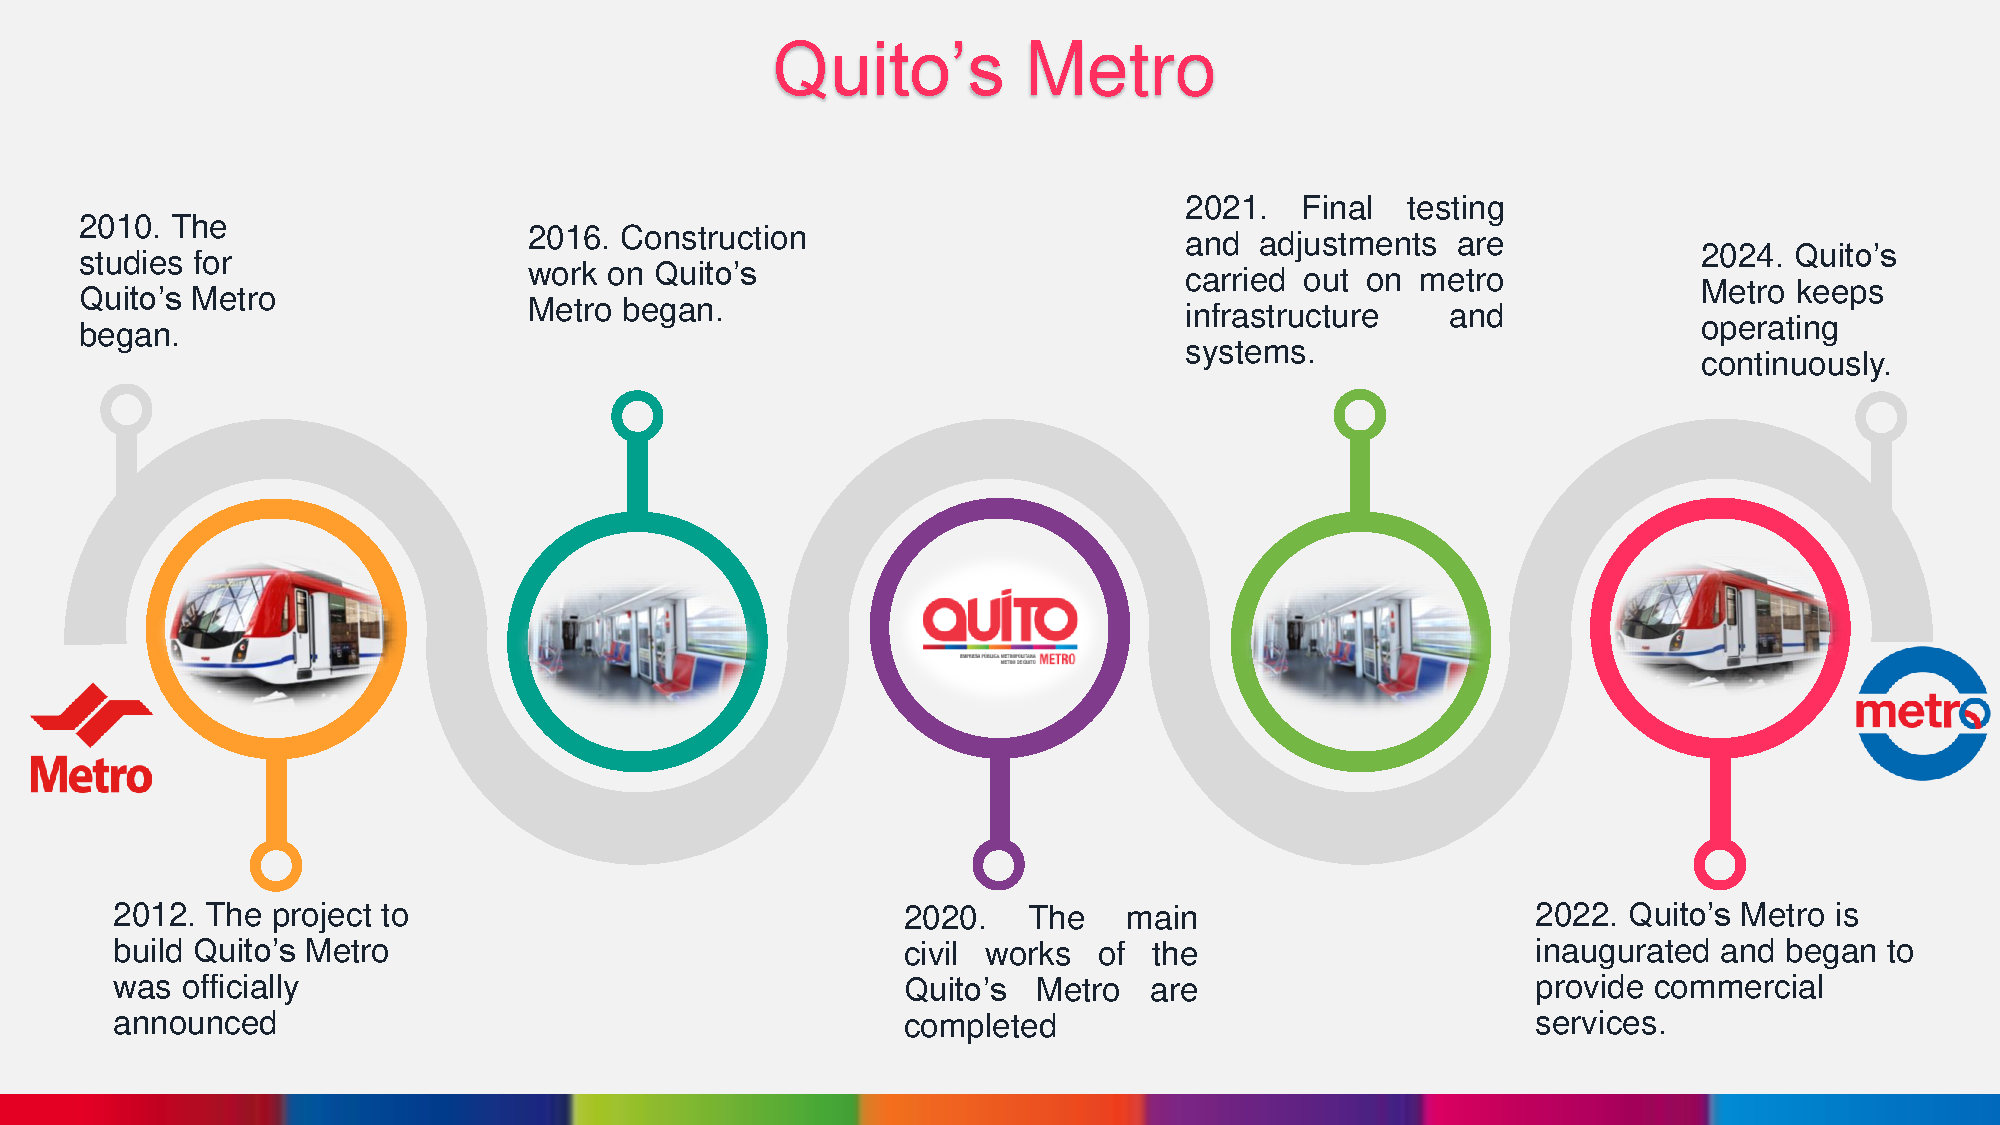
\includegraphics[width=0.4\textwidth, scale=1]{Imagenes_general/Metro de Quito_en.pdf}}
    \caption{Timeline Metro Quito}                     
    \label{Timeline Metro Quito}                                                 
\end{figure} 

Among the three projects presented, the Quito Metro is selected as the case study due to its distinction as the only one in Ecuador with an operational ATP-ATO system.

%%%%%%%%%%%%%%%%%%%%%%%%%%%%%%%%%%%%%%%%%%%%%%%%%%%%%%%%%%%%%%%%%%%%%%%%%%%%%%%%%%%%%%%%%%%%%%%%%%%%%%%%%%%%%%
%                                  Desarrollo                                                              %
%%%%%%%%%%%%%%%%%%%%%%%%%%%%%%%%%%%%%%%%%%%%%%%%%%%%%%%%%%%%%%%%%%%%%%%%%%%%%%%%%%%%%%%%%%%%%%%%%%%%%%%%%%%%%%

\section{Methodology}

\subsection{ATP-CBTC Analysis}
The following analysis used the Binary Decision Diagram (BDD) \cite{b6} method to characterize processes or components in specific variables, with the objective of evaluating ATP systems and CBTC systems in metropolitan urban transportation. \\

\subsubsection{Reliability}
ATP's reliability depends on components such as balises and speed controllers for flexible operation, while CBTC ensures high adaptability and reliability through the precise execution of advanced positioning and wireless communication systems. Figure [\ref{fig:Reliability Analysis}]\\
\begin{figure}[htbp]
 \centering
        \includegraphics[width=0.4\textwidth,scale=1]{Imagenes_general/Gráfico_Reliability.jpg}
\caption{Reliability Analysis}
 \label{fig:Reliability Analysis}
\end{figure}

\subsubsection{Safety}
ATP systems depend on traditional components and driver responses for safety, while CBTC systems leverage advanced positioning and communication technologies for more autonomous operation. CBTC excels in adaptability and scalability, integrating technological advancements to enhance safety. Figure [\ref{fig:Safety Analysis}]\\
\begin{figure}[htbp]
    \centering
    \includegraphics[width=0.4\textwidth,scale=1]{Imagenes_general/Gráfico_Safety.jpg}
    \caption{Safety Analysis}
    \label{fig:Safety Analysis}
\end{figure}
\subsubsection{Capability}

ATP systems are constrained by traditional signaling and manual processes, whereas CBTC systems, with real-time sensors and robust communication, excel in automation, adaptability, and scalability for modern railway demands. Figure [\ref{fig:Capability Analysis}]\\
\begin{figure}[htbp]
    \centering
    \includegraphics[width=0.4\textwidth,scale=1]{Imagenes_general/Gráfico_Capability.jpg}
    \caption{Capability Analysis}
    \label{fig:Capability Analysis}
\end{figure}

\subsubsection{Maintenance}
ATP system maintenance is more complicated because of aging components and fixed signaling, while CBTC systems, with their modern, modular design and software reliance, facilitate easier upgrades and adaptation to new technologies through real-time communication. Figure [\ref{fig:Maintenance Analysis}]
\begin{figure}[htbp]
    \centering
        \includegraphics[width=0.4\textwidth,scale=1]{Imagenes_general/Gráfico_Maintenece.jpg}
    \caption{Maintenance Analysis}
    \label{fig:Maintenance Analysis}
\end{figure}
\subsubsection{Costs}

ATP is cost-effective due to simpler technology and basic communication needs, while CBTC is more expensive because of its advanced components and integrated systems. [\ref{fig:Costs Analysis}]\\
\begin{figure}[htbp]
    \centering
        \includegraphics[width=0.4\textwidth,scale=1]{Imagenes_general/Gráfico_costs.jpg}
    \caption{Costs Analysis}
    \label{fig:Costs Analysis}
\end{figure}

The evaluation reveals that CBTC outperforms ATP across various critical parameters, notably demonstrating superior reliability, safety, and cost-effectiveness.[\ref{fig:Analysis}]\\

An analysis of automation grades was performed, taking into account the basic train operation functions in the Quito metro system with the current ATP, as well as the feasibility of conducting a study for the implementation of CBTC as shown in Table:[\ref{tab1}]\\

\subsection{ATP-CBTC Evaluation}

\subsubsection{UGT, Grade of  Automation}

In the table of the UNE$-$EN$-$62290$-$1 standard \cite{b17}, which addresses the basic functions for determining the grades of automation, the following is analyzed: the gray columns are not in effect to the current mass transportation system in Quito, the yellow column represents the grade of automation implemented in Quito's Metro, and the green columns represent the potential CBTC system that could be implemented in metropolitan urban transport.
\begin{table}[htbp]
\small
\centering
\caption{Grades of Automation (Quito's Metro)} 
\label{tab1}
\resizebox{7cm}{!}{
\begin{tabular}{
|>{\centering\arraybackslash}p{1.5cm}|
>{\centering\arraybackslash}p{3.5cm}|
>{\centering\arraybackslash\columncolor[gray]{0.8}}p{1.7cm}|
>{\centering\arraybackslash\columncolor[gray]{0.8}}p{1.7cm}|
>{\centering\arraybackslash\columncolor[RGB]{255, 255, 153}}p{1.9cm}|
>{\centering\arraybackslash\columncolor[RGB]{153, 255, 153}}p{1.7cm}|
>{\centering\arraybackslash\columncolor[RGB]{153, 255, 153}}p{1.7cm}|
}
\hline
\multicolumn{2}{|c|}{\multirow{2}{5cm}{Basic functions of train Operation}} & GoA0 & GoA1 & GoA2 & GoA3 & GoA4\\
\cline{3-7}
\multicolumn{2}{|c|}{} & On-Sight train operation & Non-automated train & Semiautomated train operation & Driverless train operation & Unatteneded train operation\\
\hline
\multirow{3}{1.5cm}{Ensure safe movement of train}
& Ensure safe route  
& \color{red}Human Intervention & Computer assisted & Computer assisted & Computer assisted & Computer assisted\\ 
& Ensure safe separation of train 
& \color{red}Human Intervention & Computer assisted & Computer assisted & Computer assisted & Computer assisted\\
& Ensure safe speed 
& \color{red}Human Intervention & \color{red} Human Intervention & Computer assisted & Computer assisted & Computer assisted\\
\hline
Drive train & Control acceletarion and Branking & \color{red}Human Intervention & \color{red} Human Intervention & Computer assisted & Computer assisted & Computer assisted\\
\hline
\multirow{2}{1.5cm}{Supervise guideway}& 
Prevent collison with obstacles 
& \color{red}Human Intervention & \color{red} Human Intervention & \color{red} Human Intervention & Computer assisted & Computer assisted\\
& Prevent collision with persons on tracks
& \color{red}Human Intervention & \color{red} Human Intervention & \color{red} Human Intervention & Computer assisted & Computer assisted\\
\hline
\multirow{3}{1.5cm}{Supervise passenger transfer}
& Control passengers doors 
&\color{red}Human Intervention & \color{red}Human Intervention & \color{red}Human Intervention & \color{red}Human Intervention & Computer assisted\\ 
& Prevent injuries to persons between on tracks
&\color{red}Human Intervention & \color{red}Human Intervention & \color{red}Human Intervention & \color{red}Human Intervention & Computer assisted\\
& Ensure safe starting conditions 
&\color{red}Human Intervention & \color{red}Human Intervention & \color{red}Human Intervention & \color{red}Human Intervention & Computer assisted\\
\hline
\multirow{2}{1.5cm}{Operate a train}& 
Put in or take out of operation 
& \color{red}Human Intervention & \color{red} Human Intervention & \color{red} Human Intervention & \color{red} Human Intervention & Computer assisted\\
& Supervise the status of the train
&\color{red}Human Intervention & \color{red} Human Intervention & \color{red} Human Intervention & \color{red} Human Intervention & Computer assisted\\
\hline
\multicolumn{2}{|c|}{\multirow{1}{5cm}{Ensure detection and management of emergency situacions } } &\color{red}Human Intervention & \color{red} Human Intervention & \color{red} Human Intervention & \color{red} Human Intervention & Computer assisted\\
\hline 
\multicolumn{3}{r}{\multirow{2}{*}{NOT APPLY$=$ GRAY}}&\multicolumn{2}{r}{\multirow{2}{*}{ATP$\_$UIO$=$ YELLOW}} &\multicolumn{2}{c}{\multirow{2}{*}{CBTC$\_$UIO$=$ GREEN}}
\end{tabular}
}
\end{table}
\subsubsection{Headway in Railway Signaling}
The term "headway" refers to the interval between consecutive trains on the same track, crucial for the capacity and safety of rail transport. CBTC systems significantly improve headway through continuous communication between trains and the control center, real-time adjustable virtual blocks, and Automatic Train Operation (ATO), optimizing frequency and capacity, as seen in the Beijing Metro, Paris Metro and Madrid Metro.\cite{b8}  In contrast, ATP systems, like those in the Metro Quito and Metro Lima, have a higher and less efficient headway\cite{b9} \cite{b10}.\\ 

\textbf{Research:}
This research utilized verifiable data from official sources on current rolling stock and incorporated data from the Quito Metro project\cite{b11}. Considering train specifications, system requirements\cite{b17}, and applicable regulations\cite{b16}, calculations were performed using Universidad Politécnica de Madrid software to simulate the project's conditions\cite{b4}.\\

\textbf{Conditions:}
These conditions include fundamental parameters such as tractive effort, effective power, maximum braking force, and line operating speed. Tractive effort is the maximum force a train can apply to move and accelerate as shown in Equation:\\

Tractive effort \cite{b16}:
\begin{equation}
\scalebox{0.9}{$
F_{\text{max,c}} = \frac{P_{c} \cdot 100 \cdot 3.6}{V}   
$}
\label{ec:FT}
\end{equation}
\begin{itemize}
    \item $F_{\text{max,c}}$ is the continuous traction effort, 82.08 kN.
    \item $P_{c}$ is the continuous power of the motors, 570 kW. 
    \item $V$ is the speed of the train, 100 km/h.
\end{itemize}
Effective power denotes the engine's ability to maintain motion under varying loads and resistance as shown in Equation:\eqref{ec:FT}. Maximum braking force reflects the train's capacity to decelerate safely and efficiently, while line operating speed specifies the maximum speed for normal service conditions\cite{b16}.
\begin{table}[htbp]
\caption{Simulation cases}
\label{table:simulations}
\centering
\resizebox{8cm}{!}{
\begin{tabular}{|c|c|c|c|c|}
%\toprule
\hline
\rowcolor[gray]{0.9}
N° & \begin{tabular}[c]{@{}c@{}}Station \\ stopping \\ time [sec]\end{tabular} & \begin{tabular}[c]{@{}c@{}}Headway \\ $[min]$\end{tabular} & \begin{tabular}[c]{@{}c@{}}N° \\ Trains\end{tabular} & Name\_Simulation \\ %\midrule
\hline
SIM-1  & 30 & 2   & 18 & \scriptsize SIM-1\_TIME-30\_HW-2\_TRAINS-18\\ 
\hline
SIM-2  & 30 & 2   & 19 & \scriptsize SIM-2\_TIME-30\_HW-2\_TRAINS-19\\
\hline
SIM-3  & 30 & 1.5 & 23 & \scriptsize SIM-3\_TIME-30\_HW-1.5\_TRAINS-23\\
\hline
\textbf{SIM-4}  & \textbf{25} & \textbf{2}   & \textbf{18} & \scriptsize \textbf{SIM-4\_TIME-25\_HW-2\_TRAINS-18}\\
\hline
SIM-5  & 25 & 2   & 19 & \scriptsize SIM-5\_TIME-25\_HW-2\_TRAINS-19\\
\hline
SIM-6  & 25 & 1.5 & 18 & \scriptsize SIM-6\_TIME-25\_HW-1.5\_TRAINS-18\\
\hline
SIM-7  & 25 & 1.5 & 23 & \scriptsize SIM-7\_TIME-25\_HW-1.5\_TRAINS-23\\
\hline
\textbf{SIM-8}  & \textbf{25} & \textbf{1.5}&\textbf{24}&\scriptsize\textbf{SIM-8\_TIME-25\_HW-1.5\_TRAINS-24}\\
\hline
\textbf{SIM-9}  & \textbf{25} & \textbf{2}&\textbf{16}&\scriptsize\textbf{SIM-9\_TIME-25\_HW-2\_TRAINS-16}\\
\hline
SIM-10 & 20 & 2   & 23 & \scriptsize SIM-10\_TIME-20\_HW-2\_TRAINS-23\\ 
\hline 
\multicolumn{5}{c}{ }
\end{tabular}
}
\vspace{0.3cm}
\begin{minipage}{\linewidth} 
\footnotesize Note: Simulation cases presented in the table will be documented in a public repository \cite{b12}. This repository will include simulation scripts and test results, organized to facilitate navigation and access to the necessary information.
\end{minipage}
\end{table}

The initial simulation conditions, detailed in Tables [\ref{table:simulations}] and [\ref{table:train_data}], include key variables such as station dwell time, headway, and the number of trains in operation. These are crucial for understanding the research. Additional simulation cases will be available in a public repository for further comparison and analysis \cite{b12}.

\begin{table}[htbp]
\caption{Train Data}
\label{table:train_data}
\centering
\resizebox{5cm}{!}{
\begin{tabular}{|c|c|c|}
\hline
\rowcolor[gray]{0.9}
\centering Name & Value & \scriptsize Reference \\ 
\hline
Train Type & \scriptsize CAF-MQ117 & \cite{b10} \\
\hline
Maximum Acceleration & 1,25 [\scriptsize m/s$^2$]  & \cite{b11}  \\
\hline
Maximum Deceleration Service Brake \scriptsize(80\%)  & \centering 1,30 [\scriptsize m/s$^2$] & \cite{b11} \\
\hline
Maximum Wheel Power  & 570,00 [\scriptsize kW] & \cite{b12} \\
\hline
Maximum Braking Power  & 671,00 [\scriptsize kW] & \cite{b12} \\
\hline
Emergency Brake Application Time  & 1,50 [\scriptsize seconds] & \cite{b11} \\
\hline
Normal Deceleration & 0,80 [\scriptsize m/s$^2$]  & \cite{b11} \\
\hline
Emergency Brake Deceleration \scriptsize(100\%) & 1,15 [\scriptsize m/s$^2$]  & \cite{b11} \\
\hline
Maximum Traction Effort  & 82,08 [\scriptsize kN] & \cite{b12} \\
\hline
Maximum Service Speed & 100,00 [\scriptsize km/h] & \cite{b11} \\
\hline
Train Mass & 169,00 [\scriptsize ton]& \cite{b11} \\
\hline
Train Mass (Maximum Load) & 288,00 [\scriptsize ton] & \cite{b11} \\
\hline
Maximum Braking Effort & 78,55 [\scriptsize kN] & \cite{b12} \\
\hline
Train Length & 109,10 [\scriptsize m] & \cite{b11} \\
\hline
Track Gauge & 1435,00 \scriptsize[mm] & \cite{b11} \\
\hline
Frequency  & 60,00 \scriptsize[Hz] & \cite{b13} \\
\hline
Minimum Theoretical Headway  & 2 [\scriptsize min]& \cite{b14} \\
\hline
Number of Trains  & 18,00 [\scriptsize units] & \cite{b14} \\
\hline
Hold time at stations & 25,00 [\scriptsize seconds] & \cite{b15} \\
\hline
\end{tabular}
}
\end{table}

\textbf{SIM-4:}
Shows a scenario with 18 trains\cite{b18}, a 2-minute interval between trains\cite{b18}, and a 25-second stop at each station\cite{b15}. This simulation is adjusted to the currently implemented ATP system design. The time interval between the departure of the last train and the arrival of the first train in the opposite direction has a sufficient margin to allow a normal operation.\\
\begin{figure}[htbp]
    \centering
    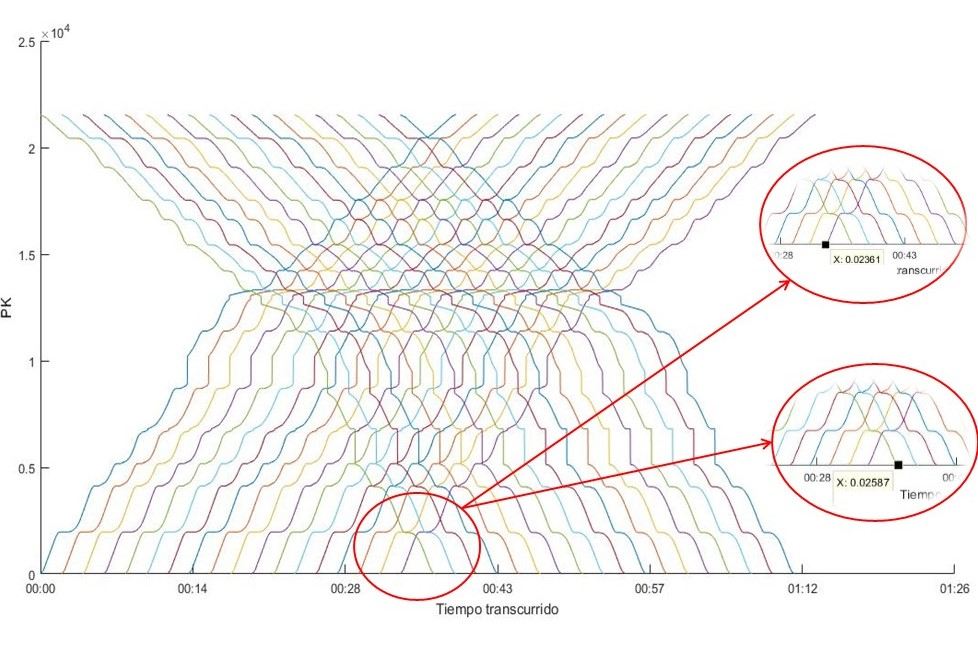
\includegraphics[width=0.35\textwidth,scale=1]{Imagenes_general/SIM-4_TIME-25_HW-2_TRAINS-18.jpg}
    \caption{Simulation with 18 trains and headway 2 mins}
    \label{fig:Simulation 4: 18 Trains / 2 mins headway}
\end{figure}

\textbf{SIM-8:}
Considers an operational scenario with 24 trains, a 1.5-minute interval between trains, and a 25-second stop at each station\cite{b15}. The time from the start of the route of the last train on the left-to-right direction presents a headway greater than the theoretical established value compared to the start time of the route of the first train in the opposite direction.
\begin{figure}[htbp]
    \centering
    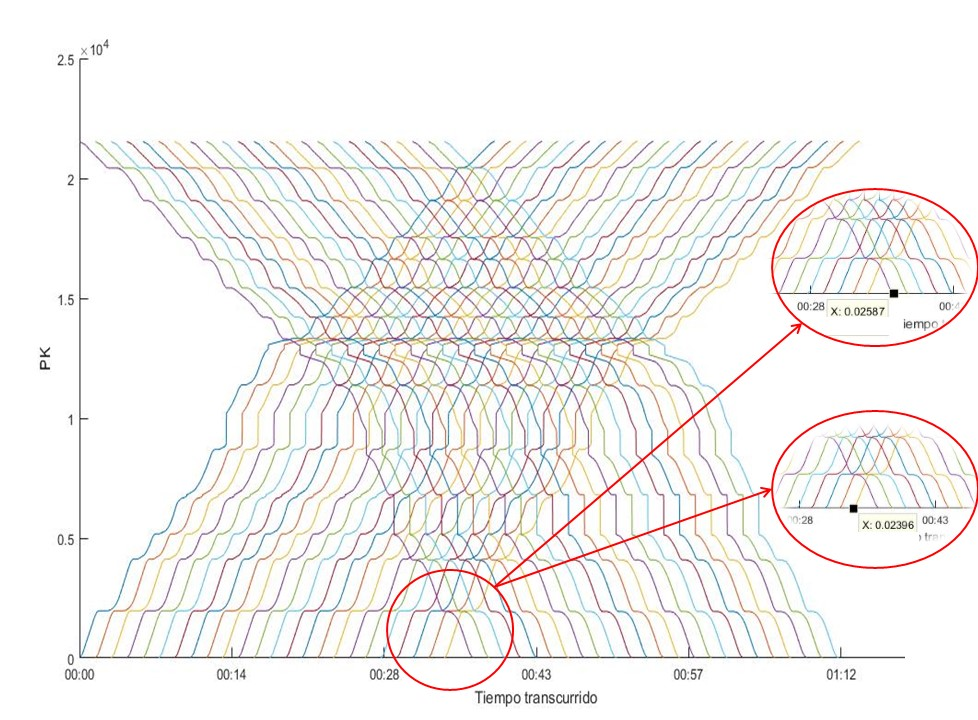
\includegraphics[width=0.35\textwidth,scale=1]{Imagenes_general/SIM-8_TIME-25_HW-1_5_TRAINS-24.jpg}
    \caption{Simulation with 24 trains and headway 1.5 mins}
    \label{fig:Simulation 8: 25 Trains / 1,5 mins headway}
\end{figure}

\textbf{SIM-9:}
Analyzes a scenario with 18 trains, of which 2 are under maintenance and 16 are in operation\cite{b20}. With a theoretical interval of 2 minutes between trains \cite{b18} and a 25-second stop at each station\cite{b15}, the simulation shows a lower train density. Under these conditions, the system can operate normally for a lower-than-expected passenger demand. This case reflects the current operational situation of the Quito Metro project\cite{b20}.
\begin{figure}[htbp]
    \centering
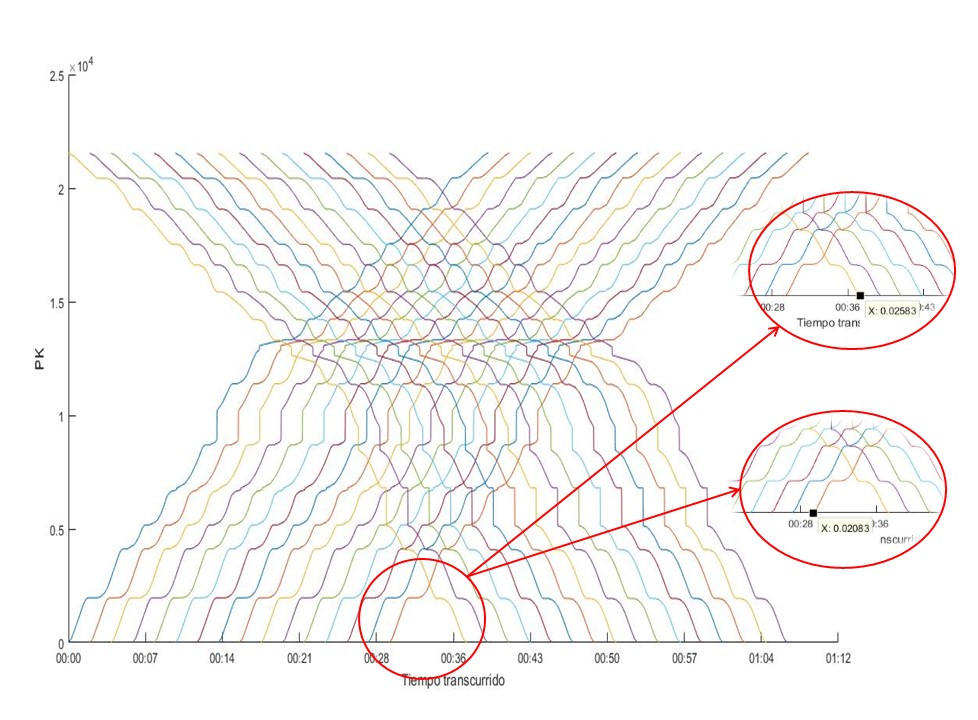
\includegraphics[width=0.35\textwidth,scale=1]{Imagenes_general/SIM-9_TIME-25_HW-2_TRAINS-16.jpg}
    \caption{Simulation with 16 trains and headway 2 mins}
    \label{fig:Simulation 9: 16 Trains / 2 mins headway}
\end{figure}

\subsubsection{Transition analysis of an ATP to a CBTC}
The transition from an ATP system to a CBTC system requires several steps and considerations to ensure capacity and safety. The key aspects of this transition are detailed below in Figure\ref{fig:Transition ATP - CBTC}:
\begin{figure}[htbp]
    \centering
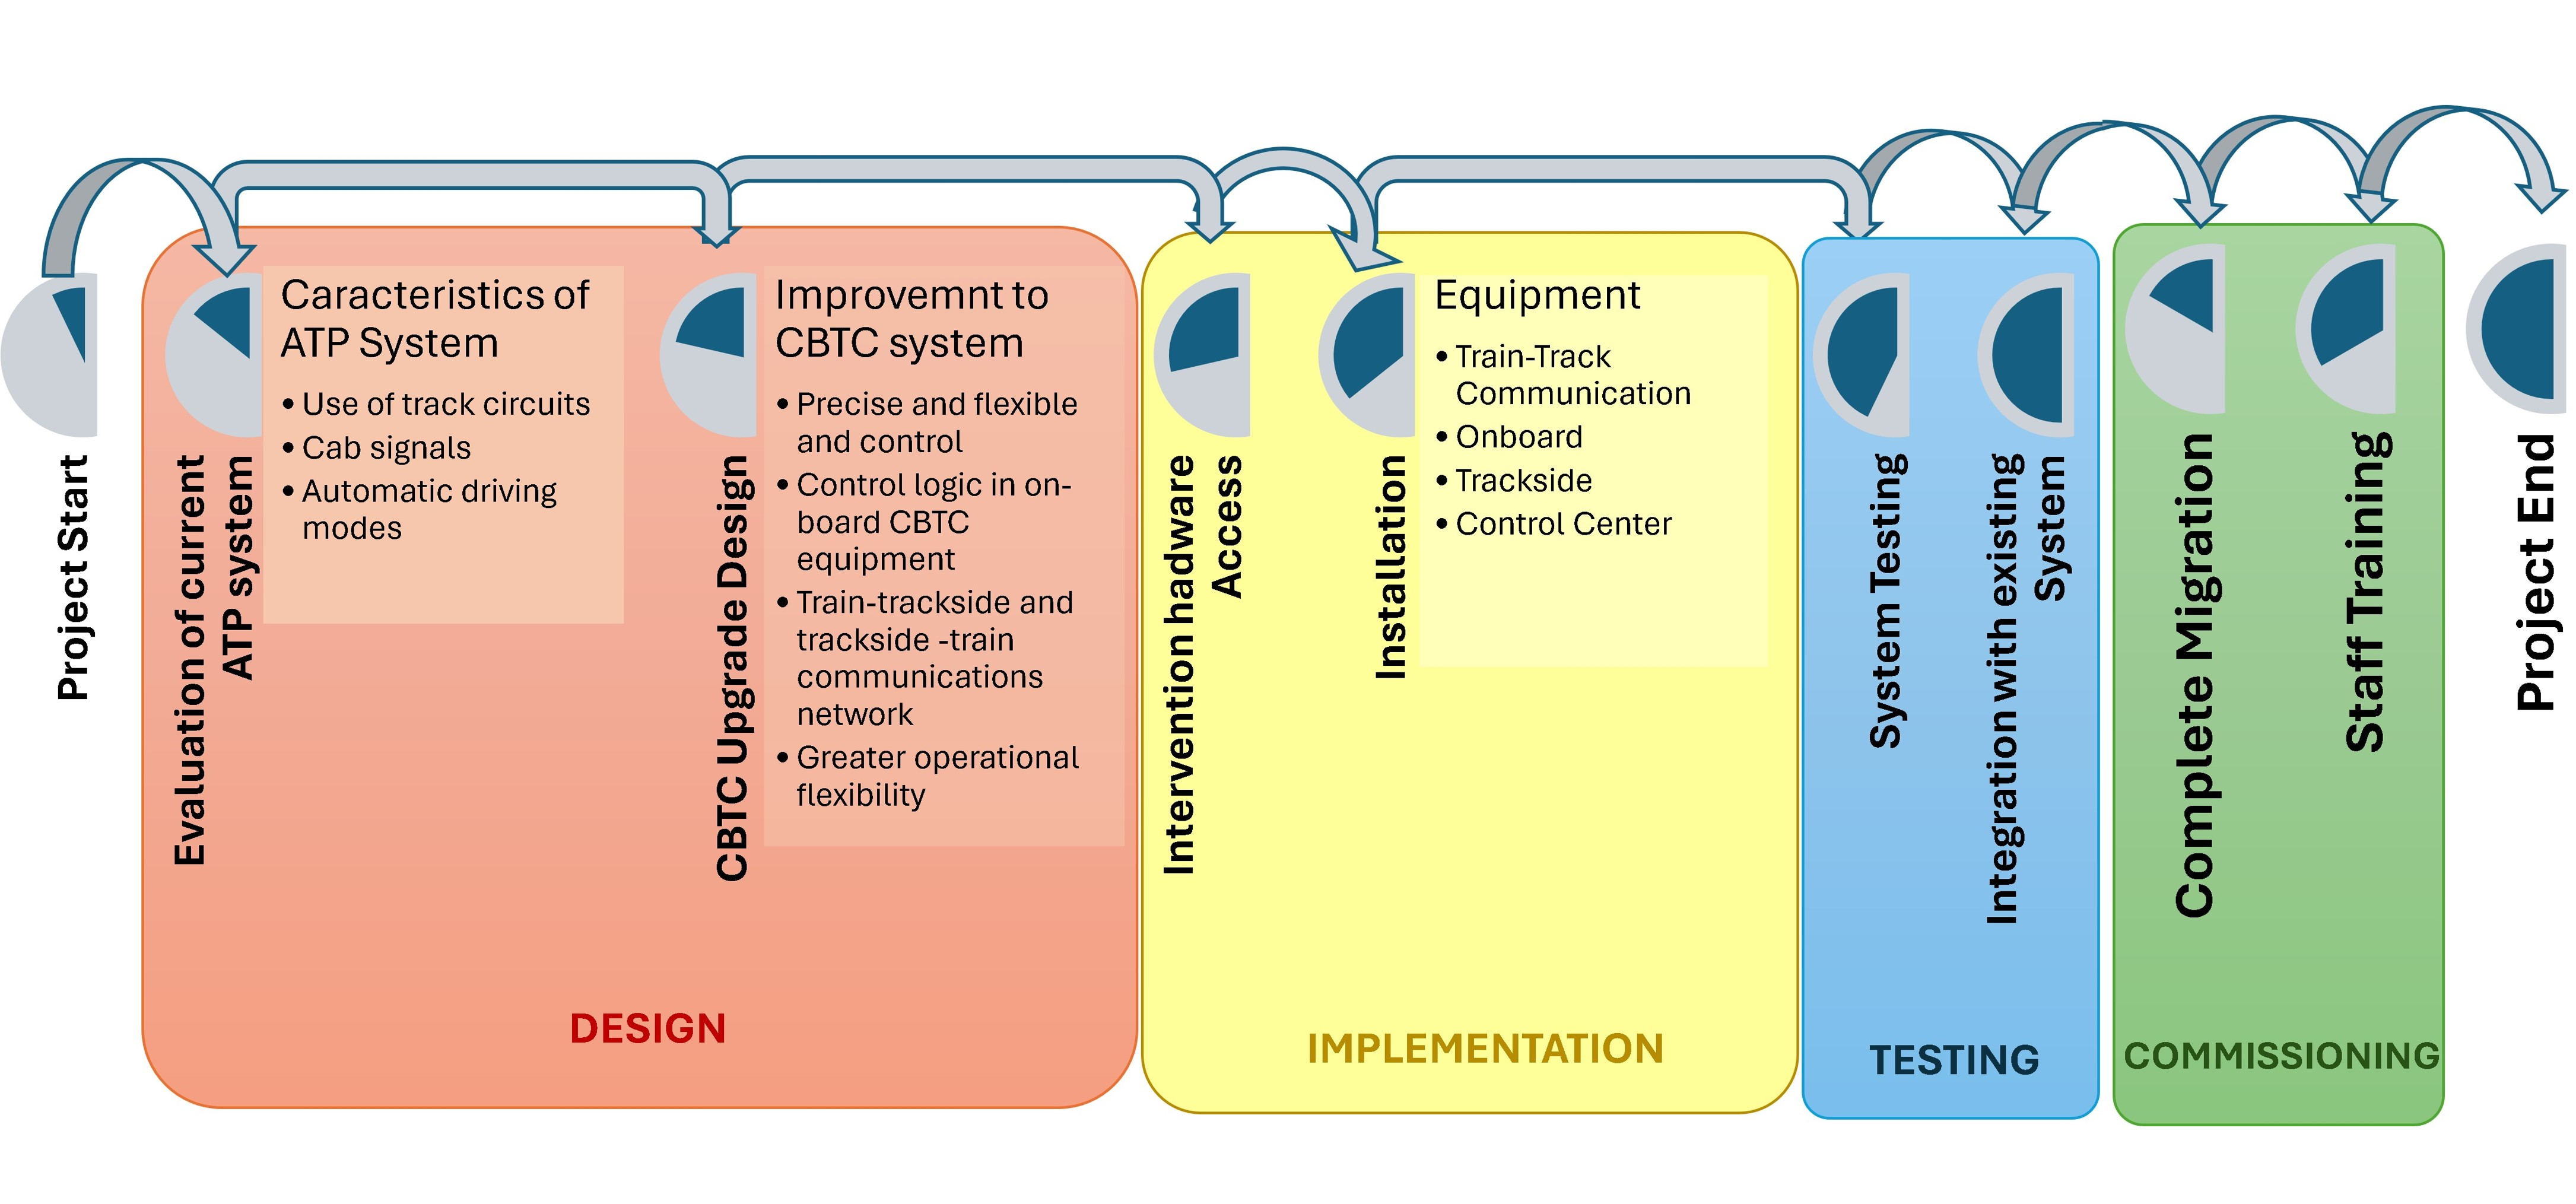
\includegraphics[width=0.45\textwidth,scale=1]{Imagenes_general/PROCESOS_TRANSITION.jpg}
    \caption{Transition ATP - CBTC}
    \label{fig:Transition ATP - CBTC}
\end{figure}
%%%%%%%%%%%%%%%%%%%%%%%%%%%%%%%%%%%%%%%%%%%%%%%%%%%%%%%%%%%%%%%%%%%%%%%%%%%%%%%%%%%%%%%%%%%%%%%%%%%%%%%%%%%%%%
%                                    RESULTADOS                                                              %
%%%%%%%%%%%%%%%%%%%%%%%%%%%%%%%%%%%%%%%%%%%%%%%%%%%%%%%%%%%%%%%%%%%%%%%%%%%%%%%%%%%%%%%%%%%%%%%%%%%%%%%%%%%%%%
\section{Results}
The importance level determined for the system analysis is as follows: reliability 30\%, safety 35\%, capacity 7\%, maintenance 10\%, and costs 18\%. The sum of these importance levels is 100\%, as shown in Figure\ref{fig:Analysis}
\begin{figure}[htbp]
    \centering
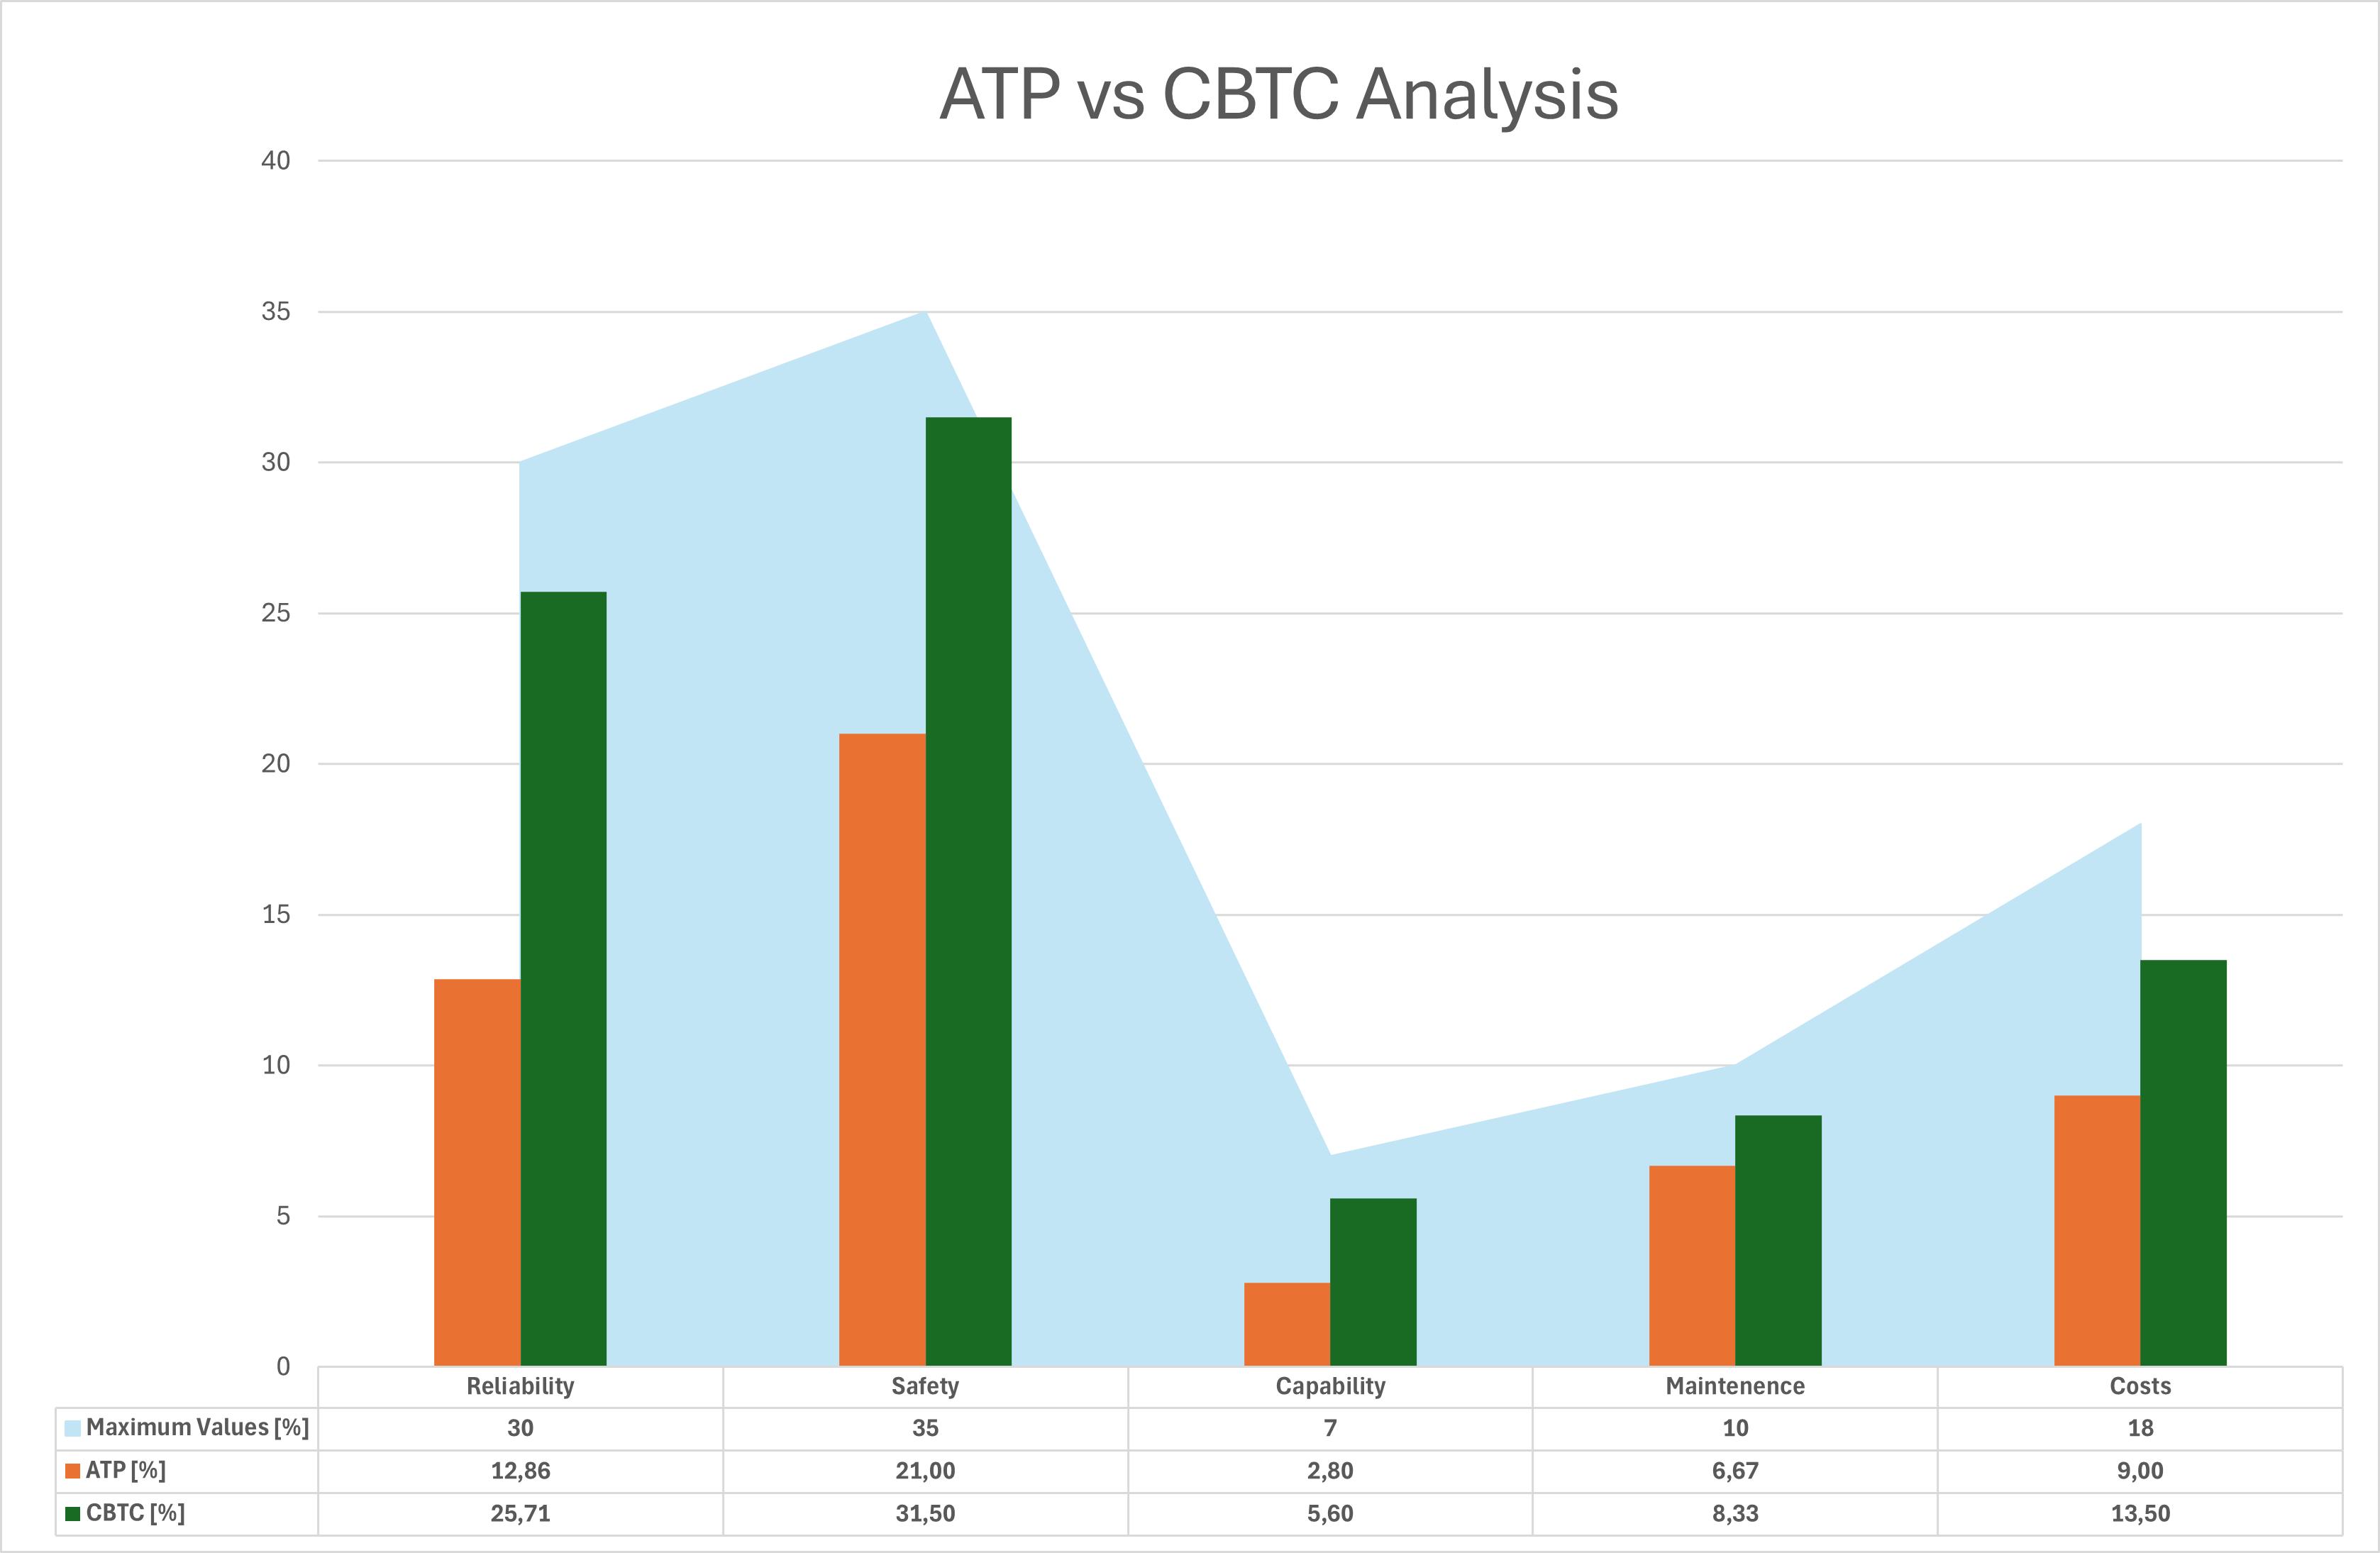
\includegraphics[width=0.4\textwidth, scale=1]{Imagenes_general/Grahp_general.png}
    \caption{ ATP and CBTC Analysis}
    \label{fig:Analysis}
\end{figure}

Different simulation cases are evaluated to determine how the system behaves in terms of headway and to optimize railway operation and traffic management with the possible implementation of CBTC in the study project as shown in Figure \ref{fig:Headway-Trains Analysis}. "Diff (min)" shows the difference in minutes between the simulated time for the last train to complete the outbound journey and the elapsed time for the first train on the return journey. "Trains Units" indicates the number of train units that could operate on the line. 
\begin{figure}[htbp]
    \centering
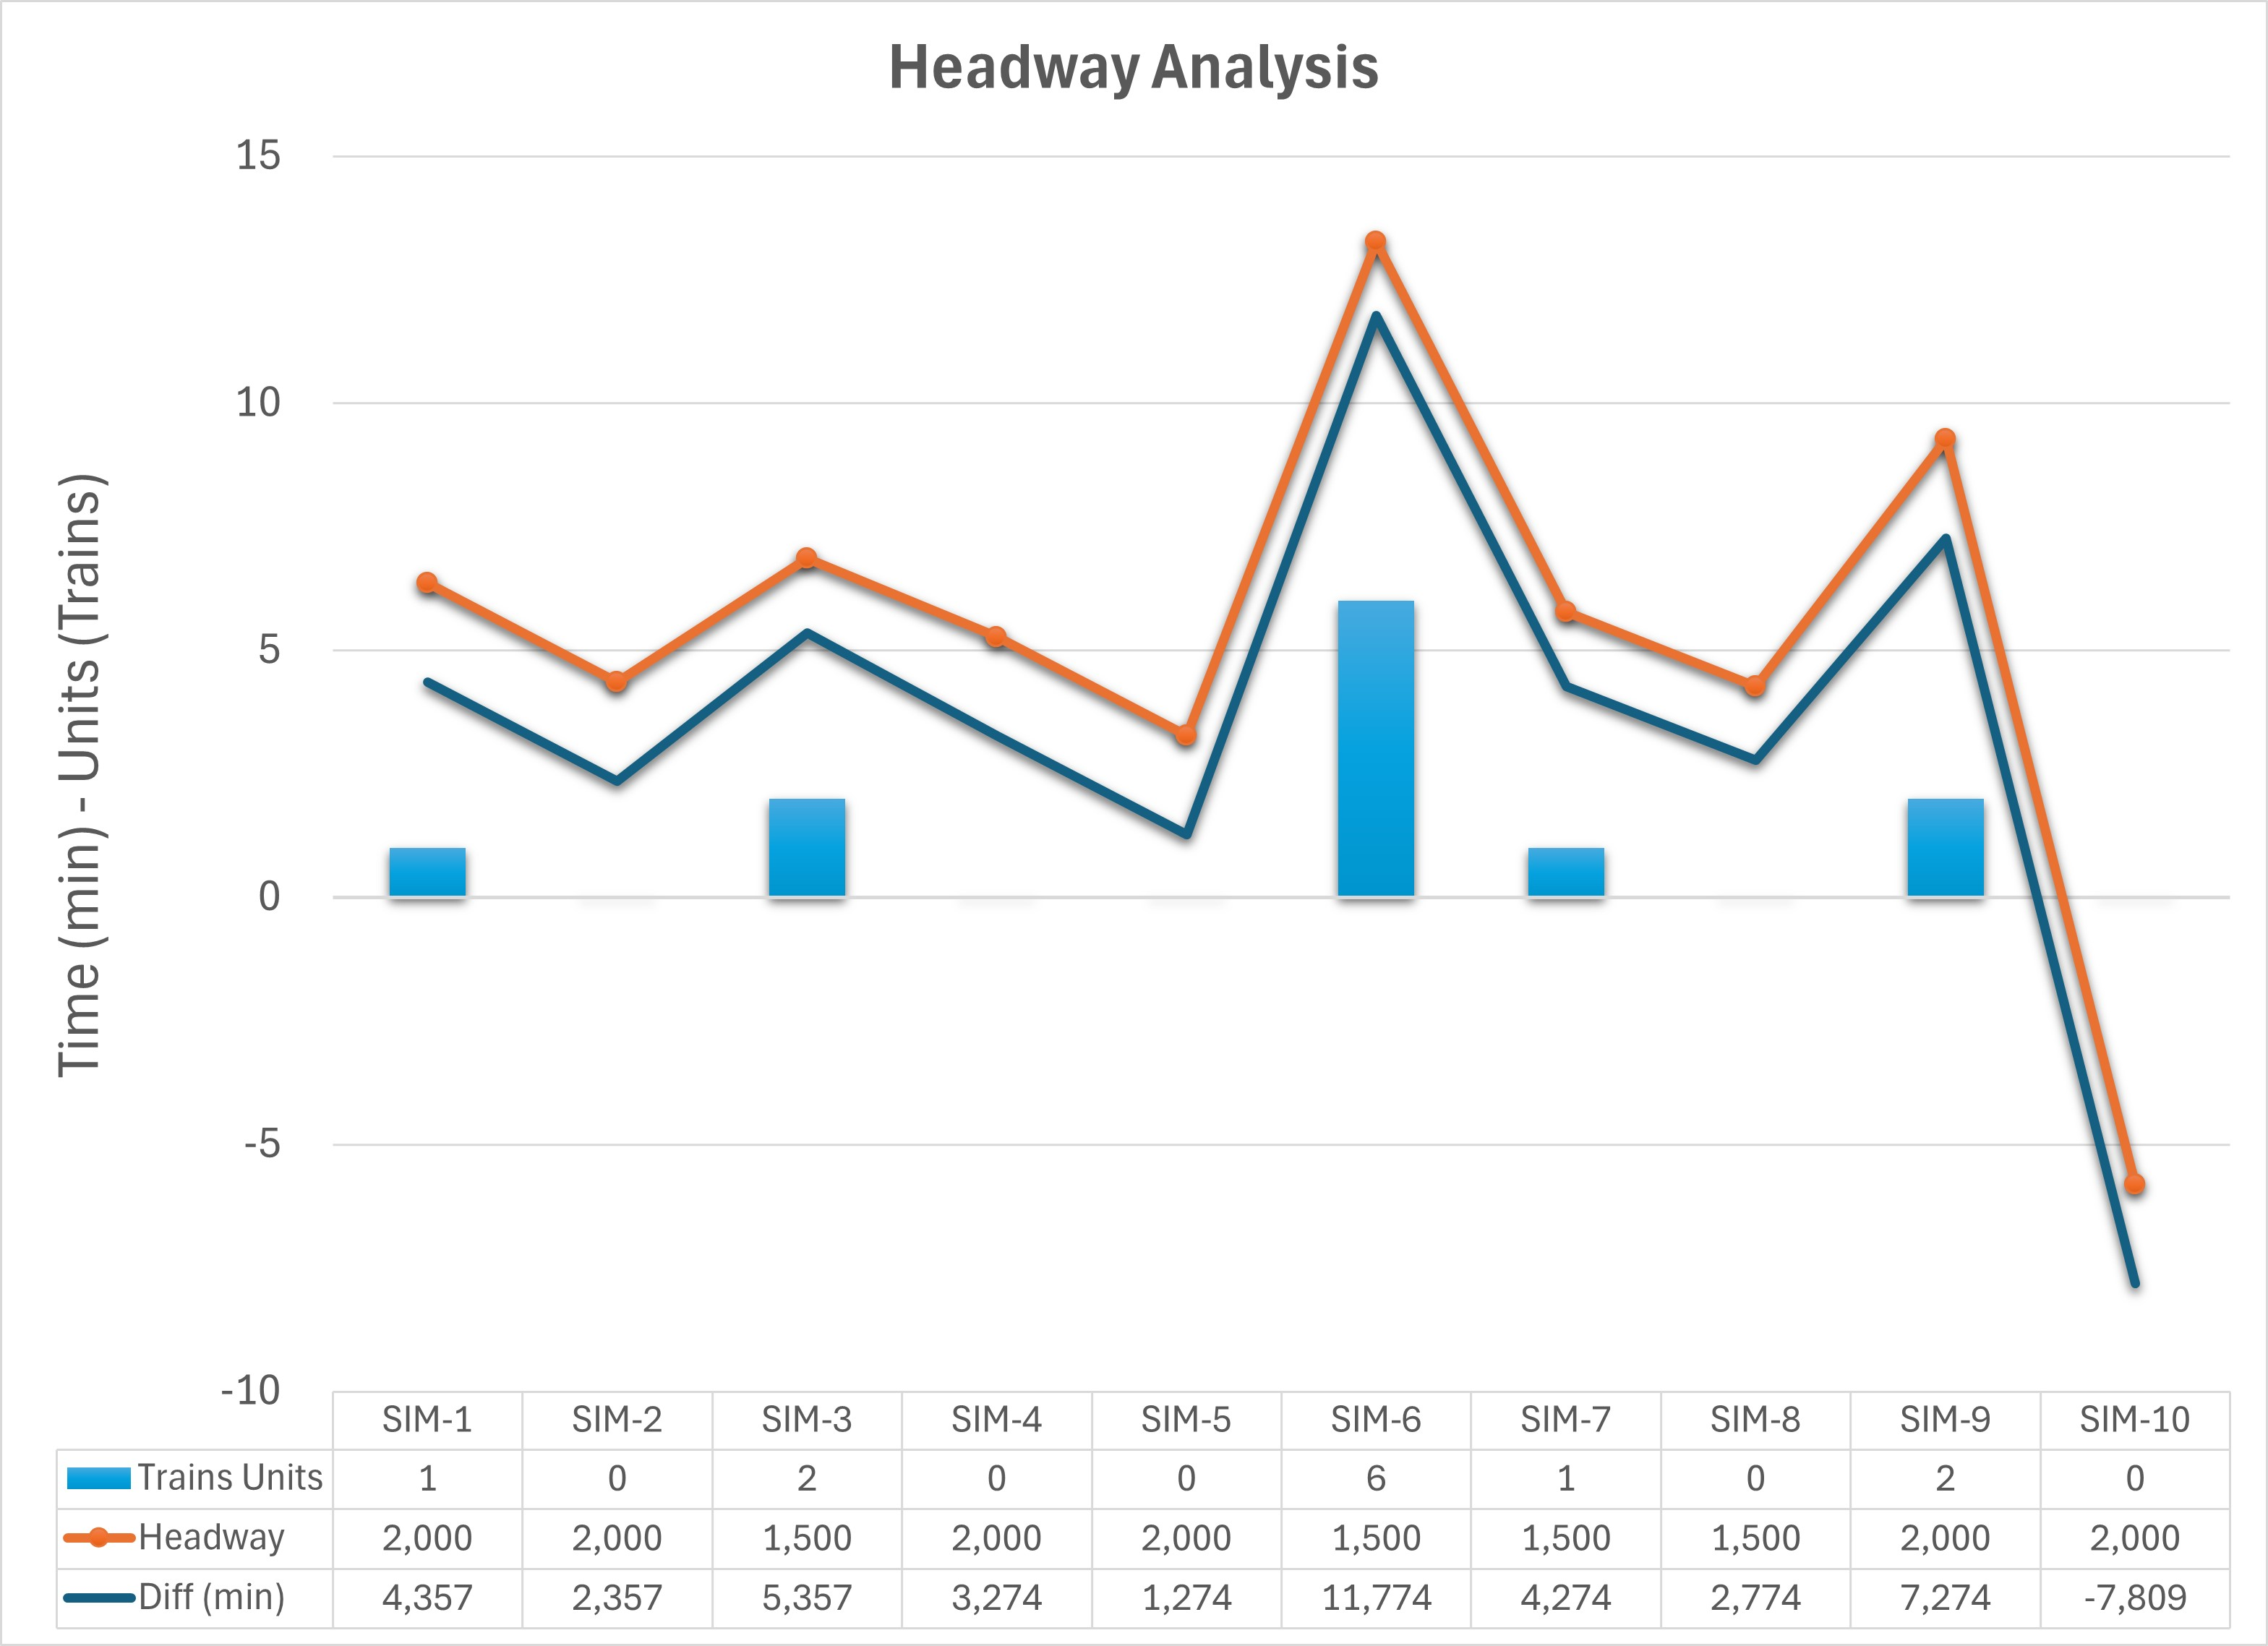
\includegraphics[width=0.4\textwidth,scale=1]{Imagenes_general/Analysis_Headway.jpg}
    \caption{Headway-Trains Analysis}
    \label{fig:Headway-Trains Analysis}
\end{figure}
The migration from ATP to CBTC improves the capacity and efficiency of the railway system through precise train localization and better traffic management, reduces the required physical infrastructure, enhances safety with automatic protection and continuous monitoring, and offers greater operational flexibility.\\

%%%%%%%%%%%%%%%%%%%%%%%%%%%%%%%%%%%%%%%%%%%%%%%%%%%%%%%%%%%%%%%%%%%%%%%%%%%%%%%%%%%%%%%%%%%%%%%%%%%%%%%%%%%%%
%                                CONCLUSIONES                                                               %
%%%%%%%%%%%%%%%%%%%%%%%%%%%%%%%%%%%%%%%%%%%%%%%%%%%%%%%%%%%%%%%%%%%%%%%%%%%%%%%%%%%%%%%%%%%%%%%%%%%%%%%%%%%%%

\section{Conclusions}
\begin{itemize}
\item The current capabilities of the railway signaling systems in Ecuador were selected for their technical complexity, impact on urban mobility, and potential for significant improvements. In the Quito Metro project, signaling is based on ATP, which includes continuous and punctual train supervision, although it still relies heavily on human intervention. The implementation of CBTC technologies alongside existing ATP could meet critical operational needs, as evidenced by the analysis results presented in Figure 15. A CBTC system outperforms ATP in terms of reliability (12. 85\%), safety (10. 5\%), capacity (2. 8\%), maintenance (1. 66\%) and costs (4. 5\%).\\

\item The adoption of the CBTC system in an environment with existing ATP in Ecuador significantly optimizes railway traffic management, increasing operational efficiency and line capacity. The CBTC reduces the interval between trains and increases line capacity, as demonstrated in case SIM-8, with 24 trains, 1.5-minute headway, and 25-second stops. Compared to case SIM-4, adjusted to the current implementation, the CBTC improves the headway by 30 seconds less than the theoretical value and increases the line by 6 trains. Surpassing the limitations of ATP, which, although it improves safety and efficiency with a GoA 2, relies more on human intervention, the CBTC allows greater operational efficiency through scalable degrees of automation and continuous communication up to the maximum GoA 4, as indicated in Table  [\ref{tab1}]\\

\item To overcome the technical obstacles in the implementation of the CBTC system in urban guided transport in Ecuador, it is recommended to conduct design studies, implementation processes, testing protocols, and commissioning as shown in Figure \ref{fig:Transition ATP - CBTC}. Additionally, develop cybersecurity protocols, project the use of artificial intelligence for predictive tasks, and apply current railway regulations. Financial obstacles will be managed through international credits, public-private partnerships, and primarily government subsidies, establishing a long-term financial plan for maintenance and updates. It is essential to conduct a cost-benefit analysis to maximize the return on investment and optimize resource allocation.
\end{itemize}
%%%%%%%%%%%%%%%%%%%%%%%%%%%%%%%%%%%%%%%%%%%%%%%%%%%%%%%%%%%%%%%%%%%%%%%%%%%%%%%%%%%%%%%%%%%%%%%%%%%%%%%%%%%%%%%%%
%                                    REFERENCIA BIBLIOGRAFÍCAS                                                  %
%%%%%%%%%%%%%%%%%%%%%%%%%%%%%%%%%%%%%%%%%%%%%%%%%%%%%%%%%%%%%%%%%%%%%%%%%%%%%%%%%%%%%%%%%%%%%%%%%%%%%%%%%%%%%%%%%

\begin{thebibliography}{00}
\bibitem{b1}IEEE Standard for Communications-Based Train Control (CBTC) Performance and Functional Requirements, IEEE Standard 1474.1, 25 February 2005.
\bibitem{b2}Ministerio de Transporte y Obras Públicas Ecuador,\textit{Proyecto "I001 Diagnóstico del Transporte Guiado a Nivel Nacional"},2021.
\bibitem{b3}Municipio de Cuenca,\textit{Especificaciones Técnicas de Obra Pública: Descripción General},2022.[Online]. Available en: \url{https://www.cuenca.gob.ec/system/files/4.11%20ESP.%20TEC.%201%20-%20DESCRIPCI%C3%93N%20GENERAL_0.pdf}
\bibitem{b4}Ar{\'a}nzazu Berbey Alvarez, Fernando Merchan, Jessica Guevara Cede{\~n}o, Alberto Cogley, and Rony Caballero,"Characterization of Line 1 of the Panama Metro," in \textit{Proceedings of the 2015 International Conference}, 2015. Figure 4. [Online]. Available: \href{https://api.semanticscholar.org/CorpusID:113501647}{https://api.semanticscholar.org/CorpusID:113501647}
\bibitem{b5} B. Ning, Ed., \emph{Advanced Train Control Systems}. Southampton, UK: WIT Press, 2010 pg 37-44.
\bibitem{b6}Farnaz Towhidi, Arash Habibi Lashkari, and Raheleh Sadat Hosseini, "Binary Decision Diagram (BDD)," in \textit{2009 International Conference on Future Computer and Communication}, 2009, pp. 496-499. doi: \href{https://doi.org/10.1109/ICFCC.2009.31}{10.1109/ICFCC.2009.31}.
\bibitem{b7}Guang-Jun Jiang, Zong-Yuan Li, Guan Qiao, Hong-Xia Chen, Hai-Bin Li, and Hong-hua Sun, "Reliability Analysis of Dynamic Fault Tree Based on Binary Decision Diagrams for Explosive Vehicle," \textit{Mathematical Problems in Engineering}, vol. 2021, pp. 1-13, 2021. [Online]. Available: \url{https://api.semanticscholar.org/CorpusID:234833855}
\bibitem{b8} S. C. Kwok, H. K. Ho, L. Zhu, F. R. Yu, and F. Wang, \textit{Advances in Communications-Based Train Control Systems}, 1st ed. Boca Raton, FL: CRC Press, 2024, pp. 195-196.
\bibitem{b9}Línea 1 del Metro de Lima y Callao. "Portal Oficial de la Línea 1 del Metro de Lima y Callao". [Online].  Available: \url{https://www.lineauno.pe/}.[Accessed: 18-may-2024].
\bibitem{b10}CAF, "Proyecto Detalle: METRO QUITO", [Online]. Available: \url{https://www.caf.net/es/soluciones/proyectos/proyecto-detalle.php?p=284. Accessed: 18 de mayo de 2024}
\bibitem{b11}"LICITACIÓN PÚBLICA INTERNACIONAL RELI 01-2013 METRO DE QUITO-BID-CAF-BEI. PLIEGO DE PRESCRIPCIONES TÉCNICAS PARTICULARES," Metro de Quito, pp. 96, 160, 161.
\bibitem{b12} Autor:elsyv-rrivera \textit{Analyze-the-implementation-and-impact-of-CBTC-and-ATP}. Available: \url{ https://github.com/elsyv/Analyze-the-implementation-and-impact-of-CBTC-and-ATP}.[Accessed: 18-may-2024]
\bibitem{b13} "MEMORIA LICITACIÓN PÚBLICA INTERNACIONAL RELI 01-2013 METRO DE QUITO-BID-CAF-BEI, Ejecución de la primera línea del Metro de Quito, Fase 2: Construcción de las obras civiles y provisión y montaje del sistema de equipamiento e instalaciones, Componente instalaciones, Subsistema de señalización, A.T.P./A.T.O. vía-tren y A.T.S." Metro de Quito, 2019, pp. 22.
\bibitem{b14} "PRIMERA LINEA DEL METRO DE QUITO FASE II. MEMORIA DESCRIPTIVA DEL SISTEMA DE SEÑALIZACIÓN, Doc. N°: PMQ-CL1-D-SEN-GEN-GEN-MEM-6001-02D, Rev.: 02D" Metro de Quito, 2019, pp 15, 27.
\bibitem{b15} "Estructuración Técnica, Legal y Financiera del Contrato de Operación y Mantenimiento de la Primera Línea del Metro de Quito," Versión 04-190614, Documentación Interna Técnica, Jun. 2019, pp 14, 16.
\bibitem{b16} "Ministerio de Transportes, Movilidad y Agenda Urbana, Agencia Estatal de Seguridad Ferroviaria, Especificación Técnica de Circulación: Cálculo de Distancias de Frenado", 2020.
\bibitem{b17}UNE-EN 62290-1-2-3: International Electrotechnical Commission, "Railway Applications – Urban Guided Transport Management and Command$/$Control Systems" IEC 62290-1-2-3:2019
\bibitem{b18}"SISTEMA DE SEÑALIZACIÓN FERROVIARIA DE LA PRIMERA LÍNEA DE METRO DE QUITO, Doc. N°: $GEI_OM_DT_SEN_V1$, Metro de Quito, 2020, pp 5."
\bibitem{b19} Metro de Quito. "Portal Oficial de la Línea 1 del Metro de Quito". [Online]. Available: \url{https://metro-quito.com/incidente-en-la-estacion-quitumbe-del-metro-de-quito/}. [Accessed: 18-may-2024].
\bibitem{b20} Primicias. "Portal Oficial del medio digital Primicias". [Online]. Available:\url{https://www.primicias.ec/noticias/quito/metro-trenes-mantenimiento-danos-contrato/}. [Accessed: 18-may-2024].



\end{thebibliography}

\end{document}

%%%%%%%%%%%%%%%%%%%%%%%%%%%%%%%%%%%%%%%%%%%%%%%%%%%%%%%%%%%%%%%%%%%%%%%%%%%%%%%%%%%%%%%%%%%%%%%%%%%%%%%%%%%%%%%%%
%                                    FINAL DEL DOCUMENTO                                                        %
%%%%%%%%%%%%%%%%%%%%%%%%%%%%%%%%%%%%%%%%%%%%%%%%%%%%%%%%%%%%%%%%%%%%%%%%%%%%%%%%%%%%%%%%%%%%%%%%%%%%%%%%%%%%%%%%%